\section{Metadatový fingerprinting a segmentace relací}
Tato kapitola popisuje dvoufázový proces kategorizace a třídění souborů ve formátu \textbf{\ac{FITS}}. Pro správnou kalibraci a zpracování astrofotografických dat je nezbytné snímky rozdělit do logických celků (relací) a ke světelným snímkům (light frames) správně přiřadit odpovídající kalibrační data. Proces se skládá ze základní textové segmentace na základě adresářové struktury a z pokročilého seskupování pomocí extrakce metadat.
\subsection{Segmentace pomocí prefixů a sufixů v cestě k souboru}
Prvním krokem, který se provádí ihned po importu souborů skrze uživatelské rozhraní (\textbf{\acs{UI}}), je rozdělení na základě uživatelsky definované adresářové struktury. Uživatel si v aplikaci může definovat množinu prefixů nebo sufixů, podle kterých se analyzuje absolutní cesta k souboru.
Uvažujme například následující strukturu složek a souborů: 
\begin{verbatim} 
FILES/Object {OBJECT}/Session {YYYY-MM-dd}/{LIGHT/DARK/FLAT/BIAS}/*.fits 
\end{verbatim}
Konkrétní plná cesta k souboru pak může vypadat následovně: \texttt{FILES/Object M31/Session 2026-02-01/2026-02-01-00-05-13--20.00-LIGHT-NOFILTER.fits}.
Při vložení souborů se aplikují definované rozdělovače (např. prefixy \texttt{"Object "} a \texttt{"Session "}) které si uživatel nastavuje v nastavení viz Obrázek \ref{fig:prefix_suffix_settings}. 

\begin{figure}[h] 
    \centering 
    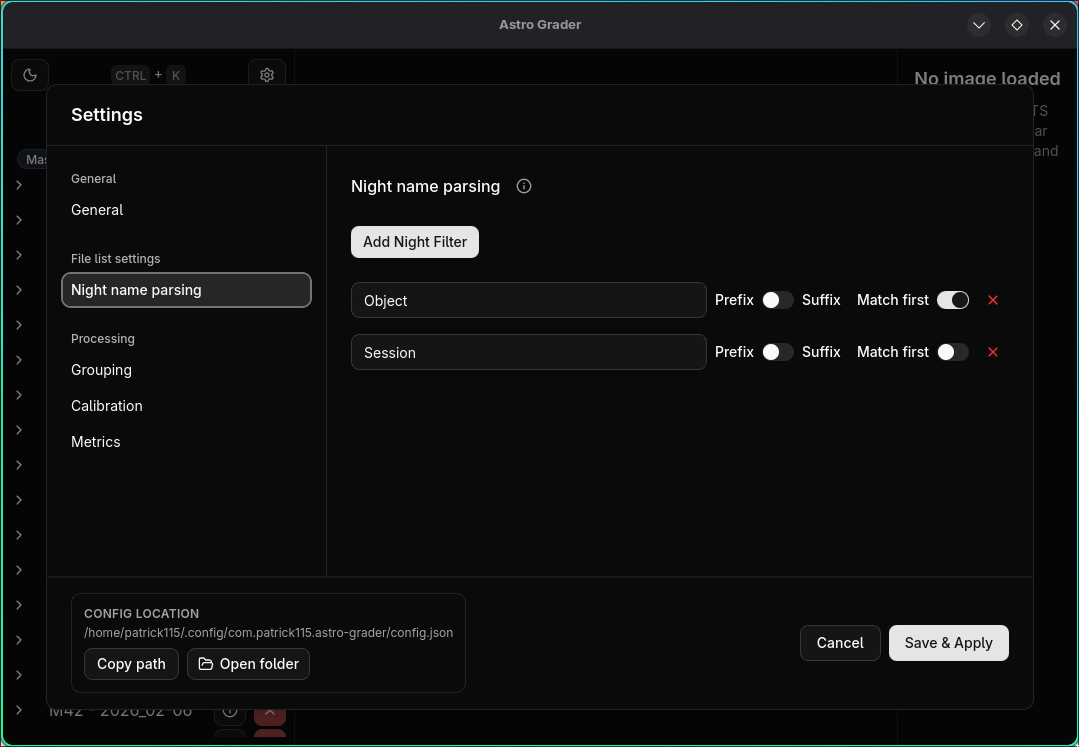
\includegraphics[width=0.8\textwidth]{assets/parsing_settings.png} 
    \caption{Ukázka nastavení prefixů a sufixů v \acs{UI} pro analýzu adresářové struktury.} 
    \label{fig:prefix_suffix_settings} 
\end{figure}

Výsledkem tohoto prvotního průchodu je logické roztřídění souborů do konkrétních pozorovacích nocí a objektů (například \texttt{M31 - 2026-02-01} nebo \texttt{Orion M42 - 2025-12-24}) viz Obrázek \ref{fig:showcase_nights}. Všechny soubory náležející dané noci a objektu jsou v rámci \acs{UI} umístěny společně. Soubory, které nevyhovují žádnému z definovaných pravidel, jsou přesunuty do kategorie \textit{Nezařazeno} (Unsorted).

\begin{figure}[h] 
    \centering 
    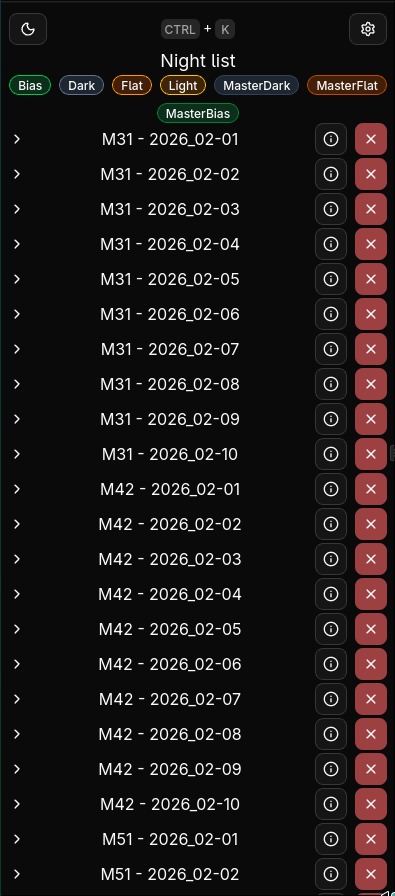
\includegraphics[width=0.4\textwidth]{assets/night_list.png} 
    \caption{Zobrazení rozdělených pozorovacích nocí a objektů po prvotním importu.} 
    \label{fig:showcase_nights} 
\end{figure}

\subsection{Seskupování a metadatový fingerprinting (Grouping)} Druhým, pokročilejším krokem je tzv. proces \textit{Grouping} (seskupování). V této fázi se analyzuje fyzický obsah hlaviček souborů \ac{FITS}, kde se čtou základní hodnoty z \ac{FITS} klíčů a tagů. Z každého snímku je tak vytvořen metadatový \uv{otisk} (tzv. fingerprint), který typicky obsahuje parametry jako: 
\begin{itemize} 
    \item \textbf{Zdrojová noc} (Source night) - odvozena z prvního kroku na základě adresářové struktury, např. M31 - 2026-02-01. 
    \item \textbf{Kamera} (Camera) - identifikována z klíčů \texttt{INSTRUME}, \texttt{CCDNAME} nebo \texttt{CAMERA}. 
    \item \textbf{Filtr} (Filter) - určující použitý optický filtr z klíče \texttt{FILTER}. 
    \item \textbf{Teleskop} (Telescope) - identifikátor optické soustavy čtený z klíčů \texttt{TELESCOP} nebo \texttt{FOCALLEN}. 
    \item \textbf{Délka expozice} (Exposure time) - hodnota expozičního času získána z klíčů \texttt{EXPTIME} nebo \texttt{EXPOSURE}. 
    \item \textbf{Zisk senzoru} (Gain) - hodnota elektronického zesílení načtena z klíčů \texttt{GAIN} nebo \texttt{EGAIN}. 
    \item \textbf{Teplota senzoru} (Temperature) - aktuální či cílová teplota čipu z klíčů \texttt{CCD-TEMP} nebo \texttt{SET-TEMP}. 
\end{itemize} 
Na základě těchto otisků a logiky definované ve zdrojových kódech aplikace se následně tvoří dedikované metadatové koše (Session Buckets), do kterých se snímky automaticky skládají.
Základem každé takové vytvořené skupiny jsou vždy \textbf{světelné snímky} (Light frames), které zůstávají zachovány ve svém zařazení do konkrétní noci z prvního kroku. K těmto světelným datům jsou následně z celého datasetu (včetně složky \textit{Nezařazeno}) algoritmicky vyhledána a přiřazena odpovídající kalibrační data: 
\begin{enumerate} 
    \item \textbf{Temné snímky (Dark frames):} Algoritmus nejprve zjišťuje, zda existuje pro danou skupinu odpovídající \textit{Master Dark} — tedy referenční snímek vzniklý statistickou integrací mnoha samostatných temných expozic, který slouží k odstranění tepelného šumu. Pokud ano, přiřadí se. V opačném případě se z noci nebo z nezařazené složky vyberou všechny jednotlivé \textit{Dark} snímky, jejichž metadata (jako expozice, zisk a teplota) korespondují se světelnými snímky dané skupiny. 
    \item \textbf{Snímky plochého pole (Flat frames):} Proces je obdobný jako u temných snímků. Upřednostňuje se případný \textit{Master Flat} — kalibrační snímek vytvořený sloučením dílčích snímků, který mapuje optické vady jako je vinětace či stíny prachových částic. Jinak se vyhledávají běžné \textit{Flat} snímky podle shody metadat (zejména zisku, případně použitého filtru a teleskopu). 
    \item \textbf{Ofsetové snímky (Bias frames):} Shodně se aplikuje logika vyhledávání \textit{Master Bias} — což je referenční obraz vzniklý složením snímků s nulovou expoziční dobou, izolující konstantní elektronický šum vygenerovaný procesem čtení dat ze senzoru — nebo běžných \textit{Bias} snímků s vyhovujícím ziskem a charakteristikou kamery. 
\end{enumerate}
Tento exaktní přístup zajišťuje, že se k dané sadě světelných snímků neomylně přiřadí pouze taková kalibrační data, která byla pořízena za odpovídajících hardwarových a teplotních podmínek, čímž je zaručen bezchybný průběh následné kalibrace.
\begin{figure}[htbp] 
    \centering 
    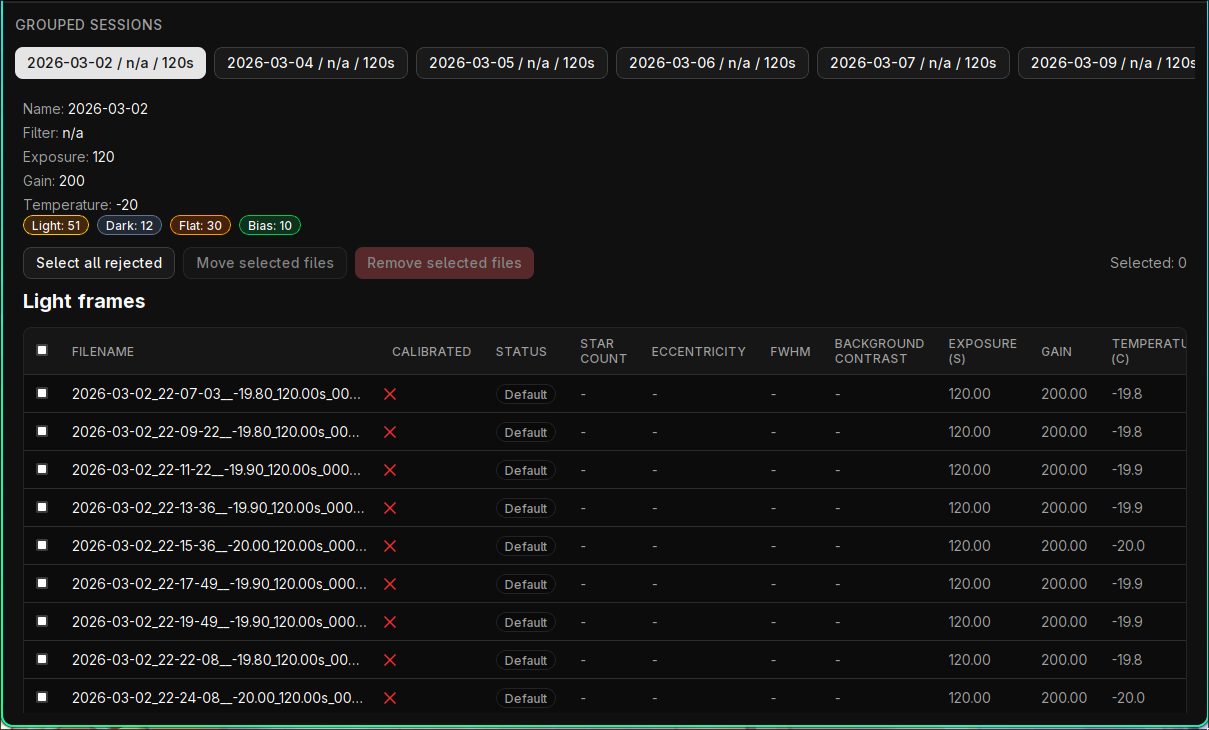
\includegraphics[width=0.8\textwidth]{assets/grouped_nights.png}
    \caption{Ukázka finálně sestavených skupin (Groups) obsahujících světelné snímky a k nim matematicky spárovaná kalibrační data na základě metadatového fingerprintingu.} 
    \label{fig:showcase_groups} 
\end{figure}